\documentclass{beamer}
\usepackage{tikz}
\graphicspath{ {./images/} }
\usepackage[usenames, dvipsnames]{color}
\usepackage[utf8]{inputenc}
\usepackage[english]{babel}


\begin{document}

\title{Visual Pollution}
\author{Gokul K}
\date{October, 2019}

\begin{frame}
    \titlepage
\end{frame}

    \begin{frame}{What is Visual Pollution}

        \begin{columns}
            \column{.5\textwidth}
                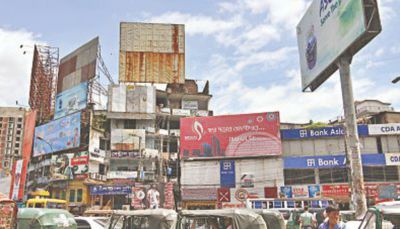
\includegraphics[height=.79\textwidth,width=.99\textwidth]{img/vp.jpg}
            \column{.5\textwidth}
            \begin{itemize}
                \item Visual Pollution is an aesthetic issue and refers to the impacts of pollution that affects ones ability to enjoy a view.  
                \item Any unwanted sights in an area can ruin its aesthetic appeal.
                \item Visual pollution affects environment by affecting the visual areas of people.
                \item The extent of visual pollution cannot be measured and is subjective.
            \end{itemize}
                
        \end{columns}
    \end{frame}

     \begin{frame}{Light Pollution}
        \begin{columns}
            \column{.5\textwidth}
                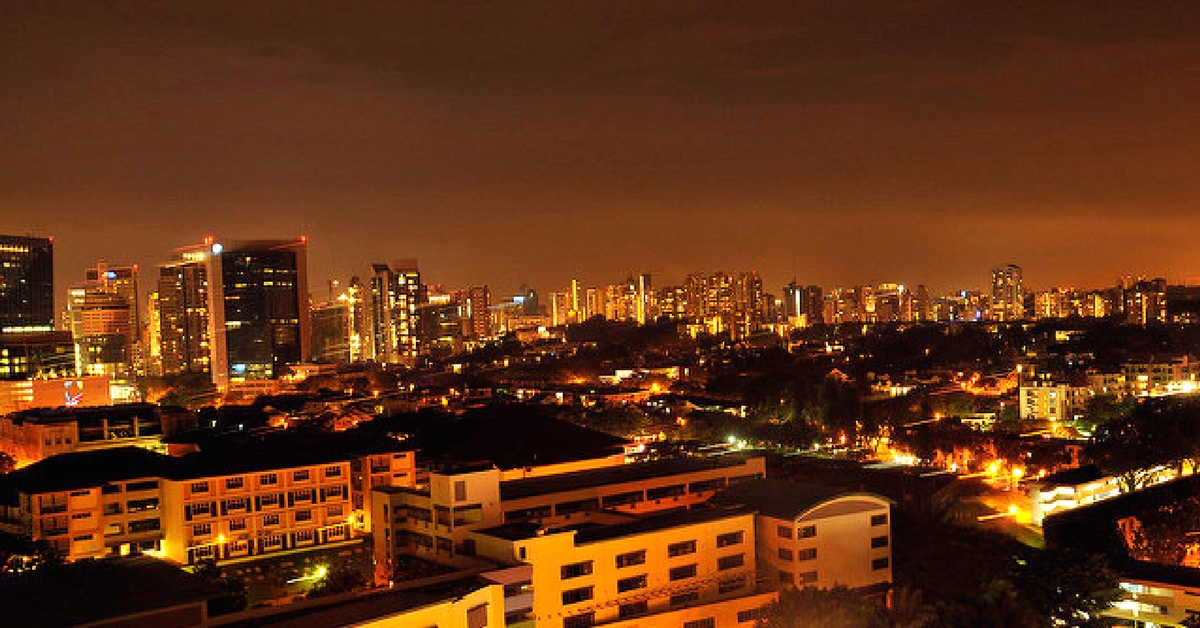
\includegraphics[height=.99\textwidth,width=.99\textwidth]{img/light-pollution.jpg}
            \column{.5\textwidth}
            \begin{itemize}
                \item Light pollution, also known as photo pollution, is the presence of artificial light in the 
            night environment.
                \item It is worsened by excessive, misdirected or obtrusive uses of light, but even 
            carefully used light fundamentally alters natural conditions.
            \item
              As a major side-effect of urbanization, 
            it is blamed for compromising health, disrupting ecosystems and spoiling aesthetic environments.
            \end{itemize}
        \end{columns}
     \end{frame}
     
     \begin{frame}
        \begin{itemize}
            \item Over the last 50 years, as countries became affluent and urbanized, demand for outdoor
             lighting increased and light pollution sprawled beyond the city limits and into suburban and
              rural areas.

        \end{itemize}
     \end{frame}

     \begin{frame}
         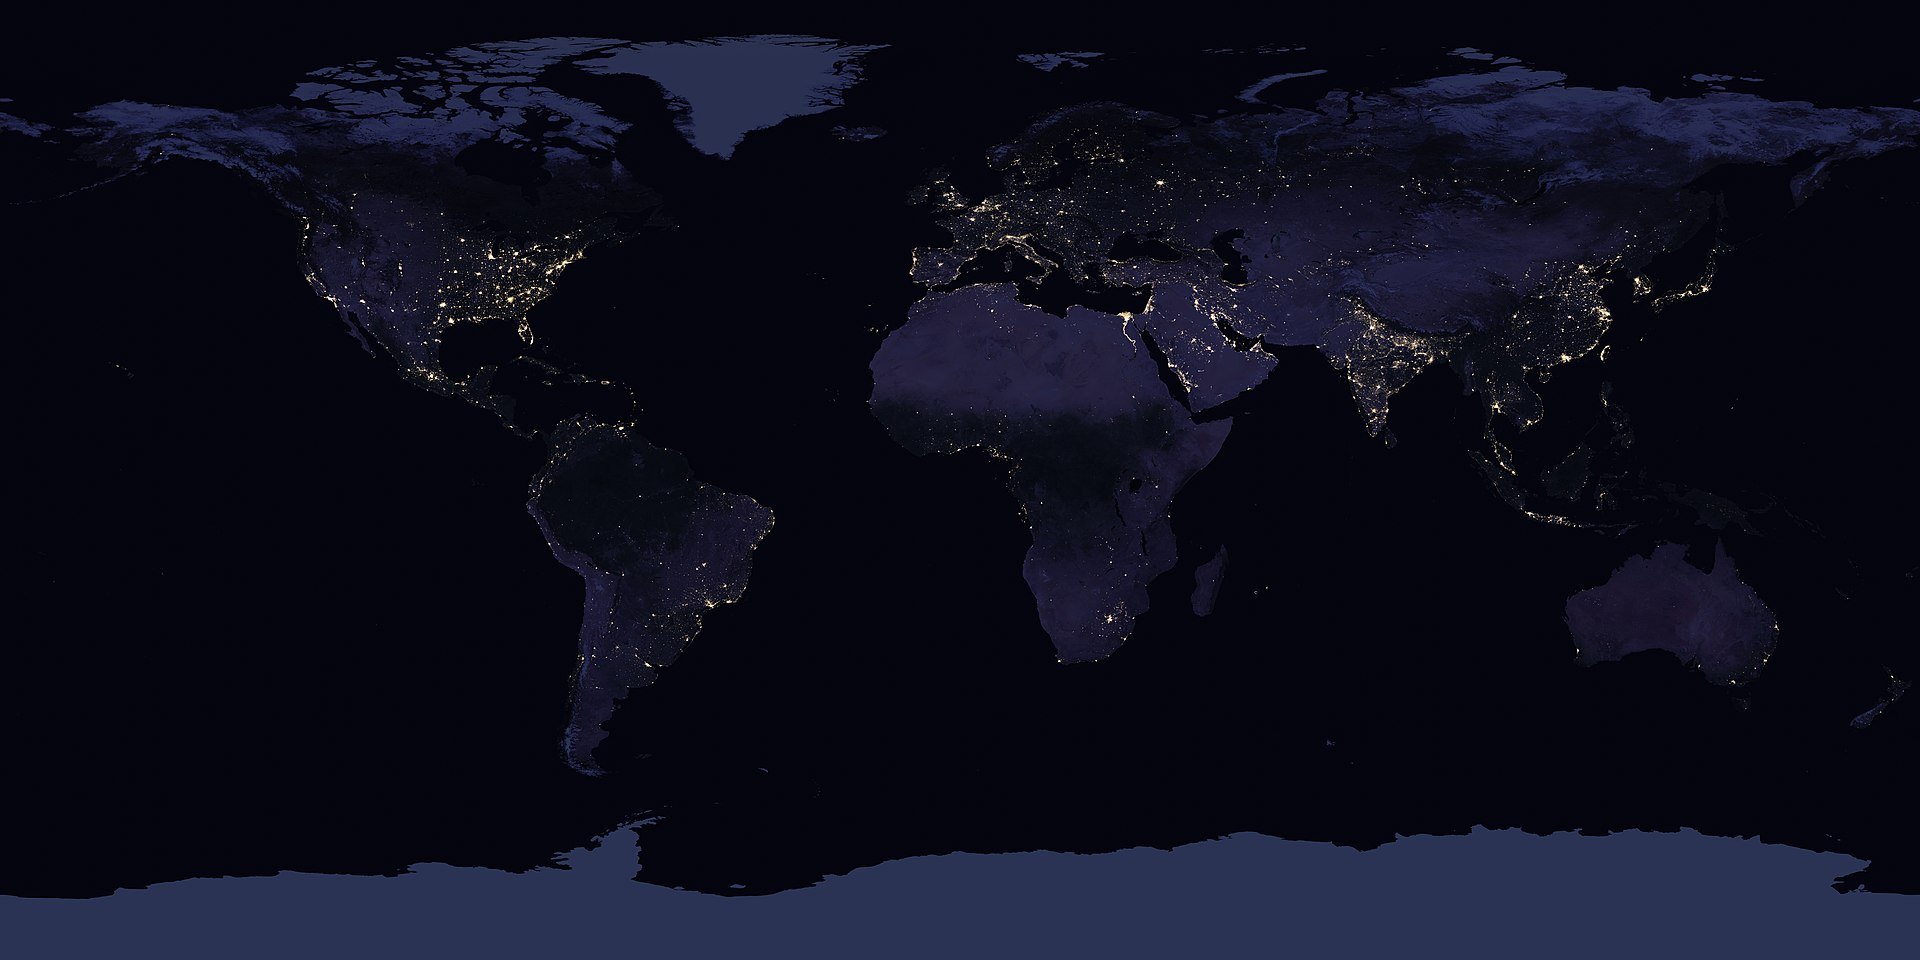
\includegraphics[height=.79\textwidth,width=.99\textwidth]{img/map.jpg}
     \end{frame}

     \begin{frame}{Causes of Visual Pollution}
        \begin{columns}
            \column{.5\textwidth}
                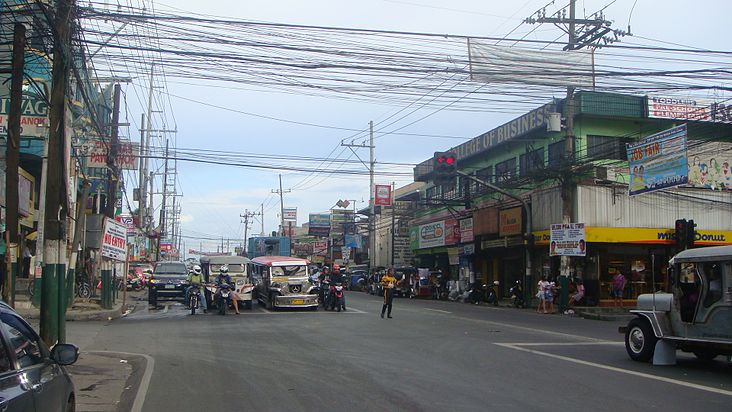
\includegraphics[height=.99\textwidth,width=.99\textwidth]{img/wiki-1.JPG}
            \column{.5\textwidth}
                \begin{itemize}
                    \item Billboards
                    \item Open storage of trash
                    \item Antennas and Electric wires
                    \item Overcrowding of an area
                    \item Irregular formations on natural and built environments
                \end{itemize}
        \end{columns}
     \end{frame}

     \begin{frame}
     \begin{columns}
        \column{.5\textwidth}
                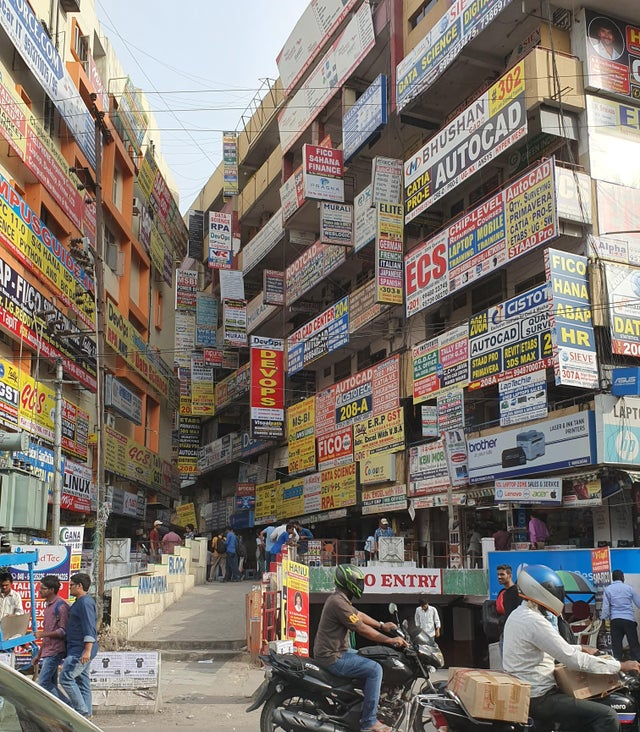
\includegraphics[height=.99\textwidth,width=.99\textwidth]{img/banners.jpg}
            \column{.5\textwidth}
            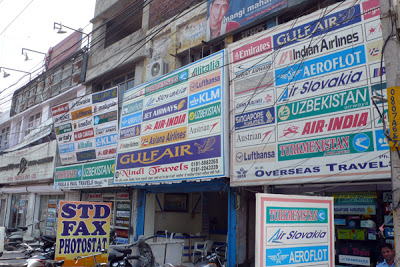
\includegraphics[height=.99\textwidth,width=.99\textwidth]{img/banners2.JPG}
        \end{columns}
     \end{frame}
    
     \begin{frame}{Reasons}
         \begin{itemize}
             \item Local managers of urban areas sometimes lack control over what is built and assembled in public places
             \item As businesses look for ways to increase the profits, cleanliness, architecture, logic and 
             use of space in urban areas are suffering from visual clutter
            \item Insensitivity of local administration is another cause for visual pollution
            \begin{itemize}
                \item Billboards, for example, have been alleged to distract drivers and clutter the land
            \end{itemize}
            \item Vandalism, in the form of graffiti or street markings made without the owner's consent.
         \end{itemize}
     \end{frame}

     \begin{frame}{Effects}
         \begin{itemize}
             \item Distaction
             \item Eye fatigue
             \item Decreases in opinion diversity
             \item Loss of identity
         \end{itemize}
     \end{frame}
     \begin{frame}
        \begin{columns}
            \column{.5\textwidth}
                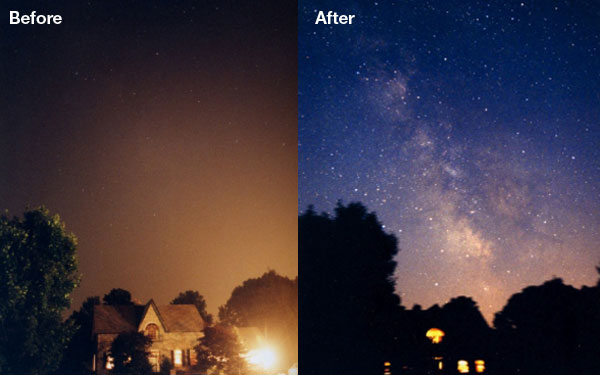
\includegraphics[height=.99\textwidth,width=.99\textwidth]{img/coreglow.jpg}
            \column{.5\textwidth}
            \begin{itemize}
                \item Many characteristics of these animals’ behavior and physiology depend on 
                the circadian rhythms, that is, the day and night influences. Hence, any amounts of 
                artificial lights introduced in their respective environments can seriously alter 
                their natural cycles and operations. 
                \item Light pollution affects the visibility of diffuse sky objects like nebulae and 
                galaxies and stars. 
                \item Wastage of energy
            \end{itemize}
        \end{columns}
     \end{frame}

     \begin{frame}
        \begin{quote}
            Visual pollution — that includes irregular formations, illegal waste dumps, billboards, unsightly cables, 
            dilapidated buildings, mounds of construction debris, ugly graffiti etc. — severely affects a person’s ability to 
            enjoy a view. This kind of pollution affects overall quality of life, reduces aesthetic appeal, economic health
             and civic-sense. In Pune, even the suburban areas are mismanaged and it is impossible to enjoy nature 
             anymore. Visual pollution not just offends the eyes, it also has an impact on the economic health 
             of a city. Ugly sights also trigger irritability. Children who grow up in such areas never learn to
             value pleasant environments. So, visual pollution has a very distinct character changing effect.
             
        -Times of India
        \end{quote}
     \end{frame}
    
     \begin{frame}{Prevention}
        \begin{columns}
            \column{.5\textwidth}
                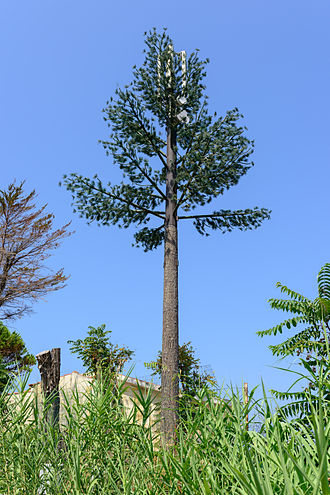
\includegraphics[height=.99\textwidth,width=.99\textwidth]{img/vp-wiki-arttree.jpg}
            \column{.5\textwidth}
                \begin{itemize}
                    \item Billboards should have specific time period after which it should be removed.
                    \item Protect trees and natural resources elements of the city, which should not be used to hang posters.
                    \item More focus on online advertisements. 
                    \item Proper solid waste management.
                \end{itemize}
        \end{columns}
     \end{frame}
     \begin{frame}
        \begin{itemize}
         \item Use certified lights at your indoor living spaces to save energy.
         \item Choose outdoor light fixtures that are shielded.
         \item Turn off lights whenever not in use
         \end{itemize}
     \end{frame}

     \begin{frame}{Conclusion}
        \begin{itemize}
            \item Visual pollution is a kind of pollution that is often overlooked
            \item Even though it may not seem so, Visual pollution can be harmful to humans and
                in general, is undesirable
            \item Ignorance makes visual pollution unmanageable
            \item With strict regulations, most of the cases of visual pollution can be avoided
        \end{itemize}
     \end{frame}

     \begin{frame}{Why I Chose this topic}
         \begin{itemize}
            \item Rarely mentioned and addressed
            \item Can be easily prevented, if the cause is man made
        \end{itemize}
     \end{frame}

\end{document}


